\apendice{Documentación de usuario}

\section{Introducción}
En el siguiente apartado se van a explicar los requerimientos de la aplicación, así como explicar cómo ejecutarla en un equipo con \emph{Windows} y las indicaciones para su correcto uso por parte del usuario.

\section{Requisitos de usuarios}

Para ejecutar la aplicación no hace falta disponer de requisitos previos, ya que se ha desarrollado un ejecutable denominado \textbf{\emph{SIM.exe}} dentro de la carpeta \emph{Aplication} del proyecto, que es capaz de arrancar la aplicación.

Por lo tanto, únicamente se necesita tener un dispositivo con sistema operativo \emph{Windows}, como se ha comentado en la sección anterior.



\section{Instalación}

No es necesaria realizar una instalación de la aplicación, ya que como se ha comentado anteriormente, se ha desarrollado un ejecutable denominado \textbf{\emph{SIM.exe}} dentro de la carpeta \emph{Aplication} del proyecto, que es capaz de arrancar la aplicación sin realizar ninguna instalación previa por parte del usuario.

Lo que sí que necesitaremos será contar con dicho ejecutable, así como la estructura de carpetas principal del proyecto.
Para obtenerlo, se puede descargar o clonar el repositorio de \emph{GitHub} desde el siguiente enlace\footnote{\href {https://github.com/mdi0007/Sistema-Informacion-sobre-Matriculacion}{www.github.com/mdi0007/Sistema-Informacion-sobre-Matriculacion}}. 


\section{Manual del usuario}

En esta sección se van a describir todas las funcionalidades de la aplicación con numerosas figuras para entender el funcionamiento de la misma.

\subsection{Creación de la Base de Datos (BBDD)}

En primer lugar es necesario crear la Base de Datos denominada BBDD donde se almacena la estructura de tablas del proyecto.
Para crearla únicamente es necesario pulsar sobre el Botón {Crear BBDD} situado en el menú superior de la aplicación, dentro de \emph{Configuración} (figura \ref{fig:crearBBDD}). Hay que destacar que este botón se ubica en el menú superior de la aplicación, ya que es un botón que se utilizará con poca frecuencia, ya que únicamente es necesario crear la BBDD la primera vez que se ejecuta la aplicación (si no tuviéramos ya creado un archivo BBDD en la ruta donde se ejecuta la aplicación). 

\begin{figure}%[!h]
		\centering
		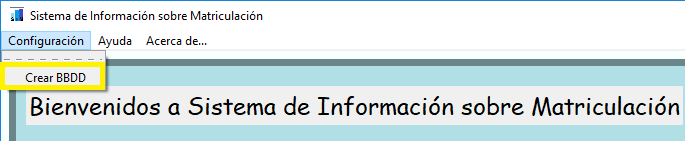
\includegraphics[width=0.9\textwidth]{crearBBDD}
		\caption{Botón de creación de la Base de Datos}\label{fig:crearBBDD}
	\end{figure}


Al pulsar sobre este botón se creará la Base de Datos y por consiguiente el fichero BBDD en la ruta donde estemos ejecutando la aplicación.
Si es la primera vez que pulsamos este botón, se creará con éxito; pero si ya existiera la BBDD, la aplicación nos mostraría un mensaje de \emph{Warning} como el de la figura \ref{fig:warningBBDD}. De esta forma, no se volverá a crear la Base de Datos y mantendremos nuestra BBDD anterior.

\begin{figure}%[!h]
		\centering
		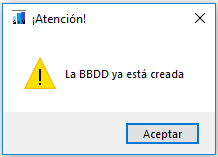
\includegraphics[width=0.5\textwidth]{warningBBDD}
		\caption{Mensaje de \emph{Warning} de BBDD ya creada}\label{fig:warningBBDD}
	\end{figure}



\subsection{Preprocesado de los ficheros Excel (.xls) descargados de \emph{Sigma}}

Una vez creada la BBDD, necesitamos introducir o meter los datos. Para esta labor, se utilizan ficheros de datos de matriculación de alumnos descargados de la aplicación \emph{Sigma}.

Ya se han explicado los problemas que existen con estos tipos de ficheros, por esta razón, se deben parsear y preprocesar antes de añadir a la BBDD. Para esta tarea, contamos con el botón de \emph{Preprocesado}. Este botón se ubica en la pantalla principal de la aplicación, ya que es un botón que se utilizará con cierta normalidad y periodicidad. 

\begin{figure}%[!h]
		\centering
		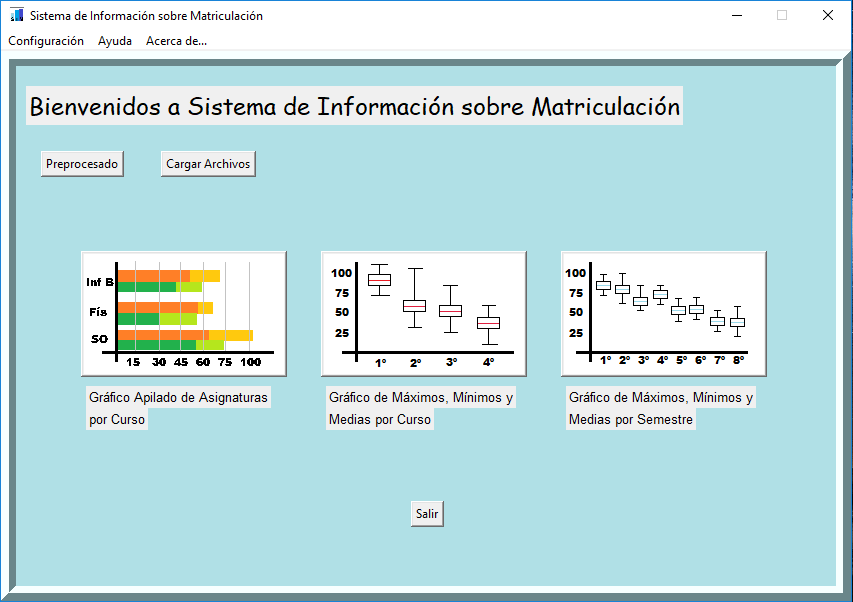
\includegraphics[width=\textwidth]{pantallaPrincipal}
		\caption{Pantalla principal de la aplicación}\label{fig:pantallaPrincipal}
	\end{figure}


Cuando pulsemos el botón de \emph{Preprocesado} (\ref{fig:pantallaPrincipal}), se mostrará una ventana del Sistema Operativo, donde se nos permitirá seleccionar archivos (.xls) únicamente (\ref{fig:ventanaSOxls}).


\begin{figure}%[!h]
		\centering
		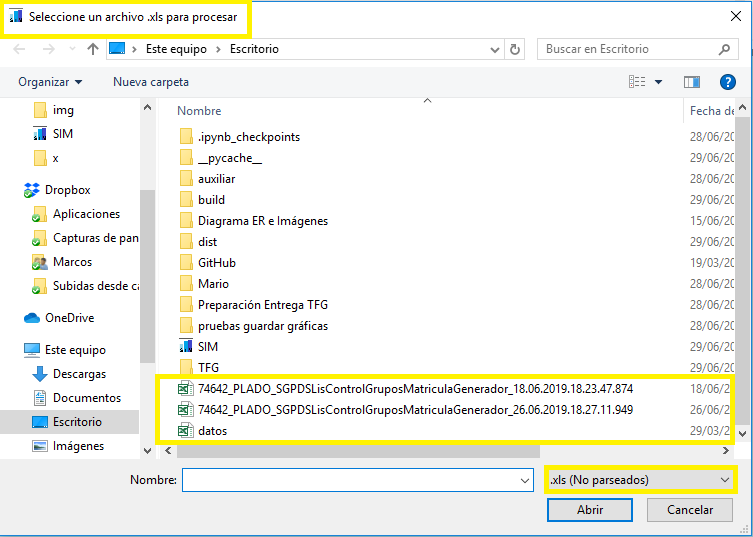
\includegraphics[width=\textwidth]{ventanaSOxls}
		\caption{Ventana del Sistema Operativo (seleccionar .xls)}\label{fig:ventanaSOxls}
	\end{figure}


Seleccionamos el archivo que deseemos (deben ser archivos descargados de \emph{Sigma}) y pulsamos abrir.
Una vez realizado esto, se generará en la misma ruta un fichero con extensión (.csv) corregido, modificado y preparado para la carga de datos en la BBDD. El resumen del proceso de preprocesado de ficheros \emph{Sigma} se puede apreciar en la figura  \ref{fig:sigmaAprocesado}.

\begin{figure}%[!h]
		\centering
		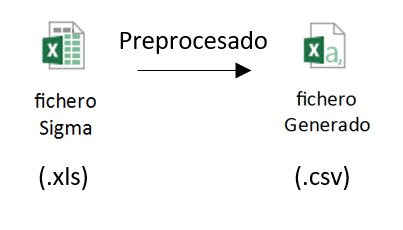
\includegraphics[width=0.5\textwidth]{sigmaAprocesado}
		\caption{Resumen de botón \emph{Preprocesado}}\label{fig:sigmaAprocesado}
	\end{figure}


\subsection{Carga de datos en la Base da Datos (BBDD)}

En este punto, ya podemos realizar la carga de datos. Para eso contamos con un botón de \emph{Cargar Archivos} situado también en la pantalla principal de la aplicación (\ref{fig:pantallaPrincipal}).

De la misma forma que el anterior paso, cuando pulsamos este botón, se mostrará una ventana del Sistema Operativo, donde se nos permitirá seleccionar archivos (.csv) únicamente (\ref{fig:ventanaSOcsv}).

\begin{figure}%[!h]
		\centering
		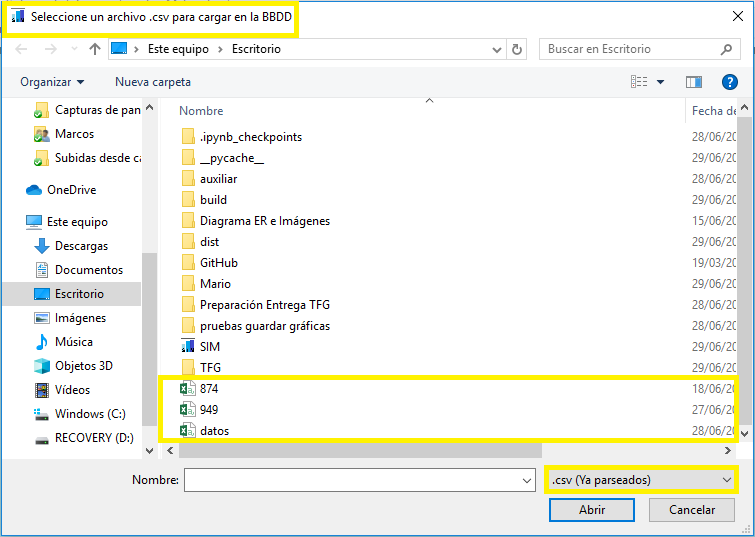
\includegraphics[width=\textwidth]{ventanaSOcsv}
		\caption{Ventana del Sistema Operativo (seleccionar .csv)}\label{fig:ventanaSOcsv}
	\end{figure}


Seleccionamos el archivo que se ha generado en el paso anterior y pulsamos abrir. Una vez realizado esto, se procederá a realizar la carga de todos los datos del fichero a la BBDD siguiendo las normas de claves primarias definidas en el modelo ER de la aplicación. El resumen del proceso de carga de datos se puede apreciar en la figura \ref{fig:procesadoABBDD}. 

\begin{figure}%[!h]
		\centering
		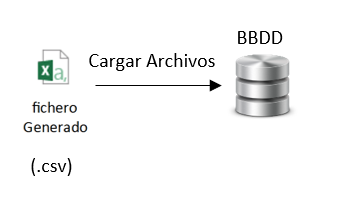
\includegraphics[width=0.5\textwidth]{procesadoABBDD}
		\caption{Resumen de botón \emph{Cargar Archivos}}\label{fig:procesadoABBDD}
	\end{figure}



\subsection{Selección y personalización de los gráficos}

En este punto, ya contamos con información o datos suficientes para realizar los diferentes tipos de gráficos.
Por lo tanto pulsamos en una de las imágenes (botones) de la pantalla principal (\ref{fig:pantallaPrincipal}) de los 3 tipos de gráficos (el primero por ejemplo) y se nos abrirá una nueva ventana (\ref{fig:ventana1}).

\begin{figure}%[!h]
		\centering
		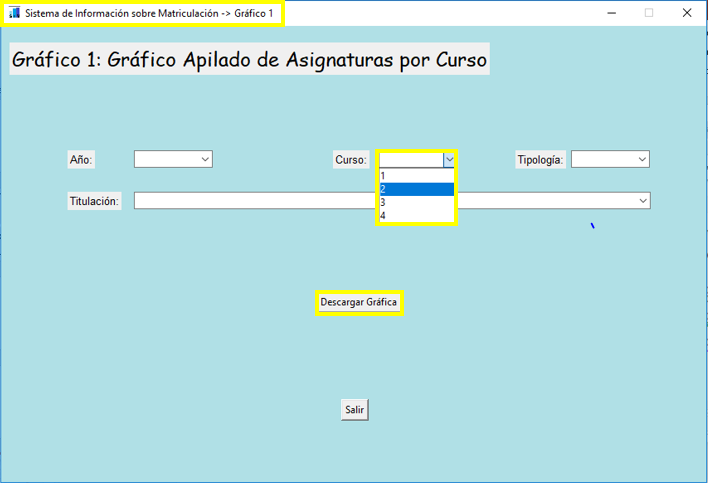
\includegraphics[width=\textwidth]{ventana1}
		\caption{Ventana secundaria para configurar el gráfico 1}\label{fig:ventana1}
	\end{figure}

En esta ventana, se muestran una serie de desplegables con la información necesaria para que el usuario seleccione y escoja los parámetros para generar el gráfico específico que desee. Hay que destacar que en cada desplegable se muestra toda la información diferente que se encuentre en la BBDD.

	
Para obtener correctamente el gráfico, es necesario seleccionar una opción de cada desplegable. En este ejemplo, es decir, en el tipo de gráfico 1, es necesario seleccionar cuatro parámetros, que son los siguientes (\ref{fig:ventana1}):


\begin{itemize}
\item \textbf{Año.} Año académico que se desea visualizar en la gráfica.
\item \textbf{Curso.} Curso que se desea visualizar. Los posibles valores son cuatro cursos (1º, 2º, 3º y 4º) en el caso de disponer de información sobre los cuatro cursos en la BBDD.
\item \textbf{Tipología.} Tipología académica que se quiere visualizar. Los posibles valores son dos tipologías (Teoría y Prácticas).
\item \textbf{Titulación.} Nombre de la titulación o plan que se desea obtener el gráfico.
\end{itemize}
   
Una vez hayamos escogido estos cuatro parámetros, podemos proceder a la descarga del gráfico.


Como se aprecia en la figura \ref{fig:ventana2}, para los tipos de gráfico 2 y 3, es necesario seleccionar únicamente dos parámetros, que ya han sido explicados anteriormente, que son:

\begin{itemize}
\item \textbf{Año.}
\item \textbf{Titulación.}
\end{itemize}
  
\begin{figure}%[!h]
		\centering
		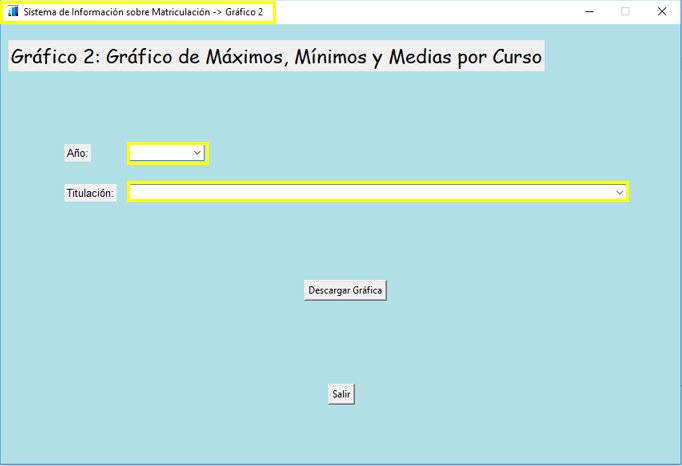
\includegraphics[width=\textwidth]{ventana2}
		\caption{Ventana secundaria para configurar el gráfico 2}\label{fig:ventana2}
	\end{figure}
	
	
\subsection{Descarga de los gráficos}

Para descargar el gráfico, únicamente debemos pulsar el botón de \emph{Descargar Gráfica} situado en las ventanas secundarias de configuración de los diferentes tipos de gráficos. Este botón se puede apreciar en las figuras \ref{fig:ventana1} y \ref{fig:ventana2}.

Una vez pulsado dicho botón se descargará la gráfica con extensión (.png) en la ruta donde estemos ejecutando la aplicación.
La nomenclatura de estos archivos es la siguiente:
 
\begin{itemize}
\item \textbf{Gráfico 1.} \emph{Grafica1} seguido de una \emph{T} (si se ha seleccionado la tipología de teoría) o una \emph{P} (si se ha escogido la tipología de prácticas), seguido de \emph{\_curso\_x} (siendo \emph{x} el tipo de curso seleccionado y por último el plan o titulación.
\item \textbf{Gráfico 2.} \emph{Grafica2\_cursos\_} seguido del plan o titulación seleccionado.
\item \textbf{Gráfico 3.} \emph{Grafica3\_semestres\_} seguido del plan o titulación seleccionado.
\end{itemize}



\subsection{Gráficos obtenidos}

Los diferentes gráficos principales que se pueden obtener gracias a la aplicación son los siguientes: \ref{fig:grafico1T}, \ref{fig:grafico1P}, \ref{fig:grafico2} y \ref{fig:grafico3}.


\begin{figure}%[!h]
		\centering
		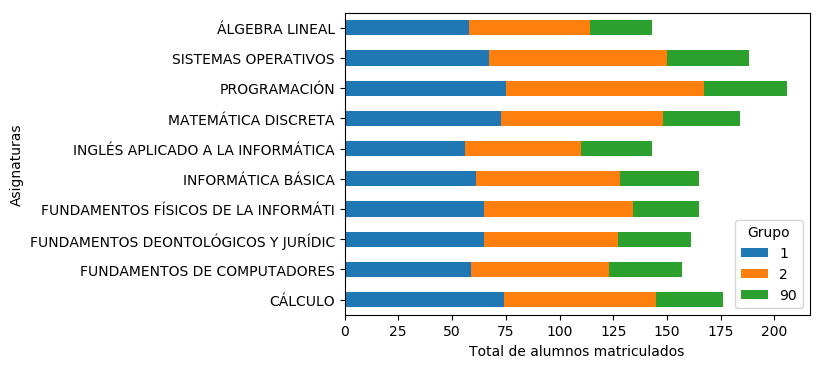
\includegraphics[width=\textwidth]{grafico1T}
		\caption{Gráfico 1: Gráfico Apilado de Asignaturas de año 2018-2019 de 1º de Grado en Ingeniería Informática de Tipología Teoría}\label{fig:grafico1T}
	\end{figure}


\begin{figure}%[!h]
		\centering
		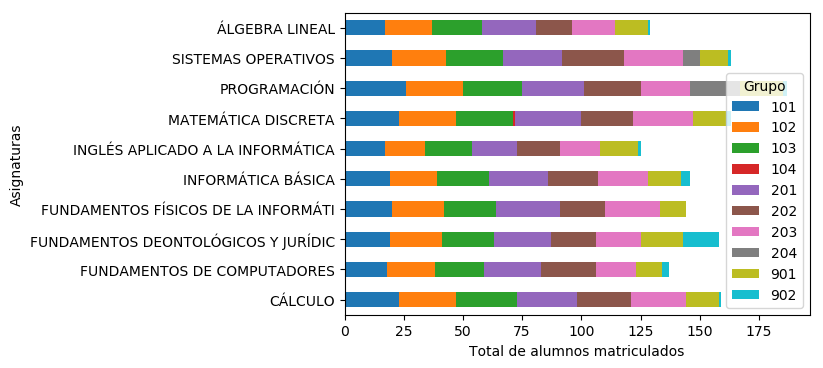
\includegraphics[width=\textwidth]{grafico1P}
		\caption{Gráfico 1: Gráfico Apilado de Asignaturas del año 2018-2019 de 1º del Grado en Ingeniería Informática de Tipología Prácticas}\label{fig:grafico1P}
	\end{figure}

\begin{figure}%[!h]
		\centering
		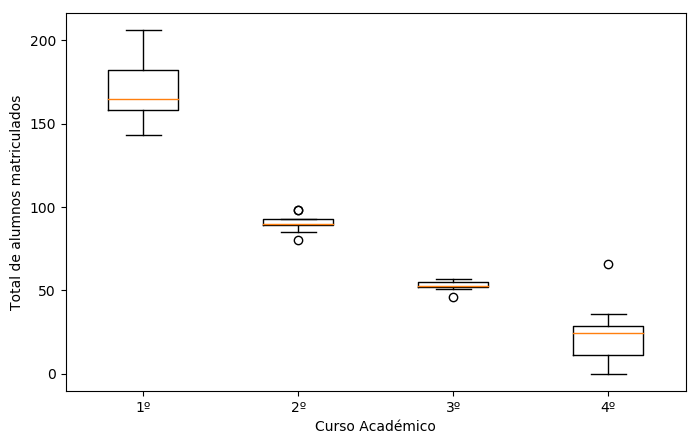
\includegraphics[width=0.8\textwidth]{grafico2}
		\caption{Gráfico 2: Gráfico Apilado de Máximos, Mínimos y Medias por Curso del año 2018-2019 del Grado en Ingeniería Informática}\label{fig:grafico2}
	\end{figure}

\begin{figure}%[!h]
		\centering
		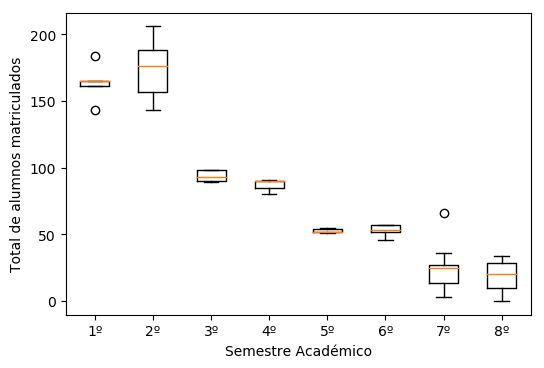
\includegraphics[width=0.8\textwidth]{grafico3}
		\caption{Gráfico 3: Gráfico Apilado de Máximos, Mínimos y Medias por Semestre del año 2018-2019 del Grado en Ingeniería Informática}\label{fig:grafico3}
	\end{figure}


\subsection{Otras funcionalidades}

Hay que señalar que la aplicación cuenta con una opción de \emph{Ayuda} en el menú superior. Al pulsar este botón se desplegarán dos opciones (\emph{Ayuda Local} y \emph{Ayuda Web}) como se aprecia en la figura \ref{fig:ayuda}. Si pulsamos la primera opción, nos abrirá el (.pdf) de ayuda que se incorpora en la aplicación; y si pulsamos la segunda opción nos abrirá el mismo (.pdf) de ayuda pero dicho archivo se encuentra subido en el repositorio de GitHub. De esta manera, mediante esta segunda opción, se podría actualizar la información relevante a la \emph{Ayuda} de manera inmediata para el usuario.

\begin{figure}%[!h]
		\centering
		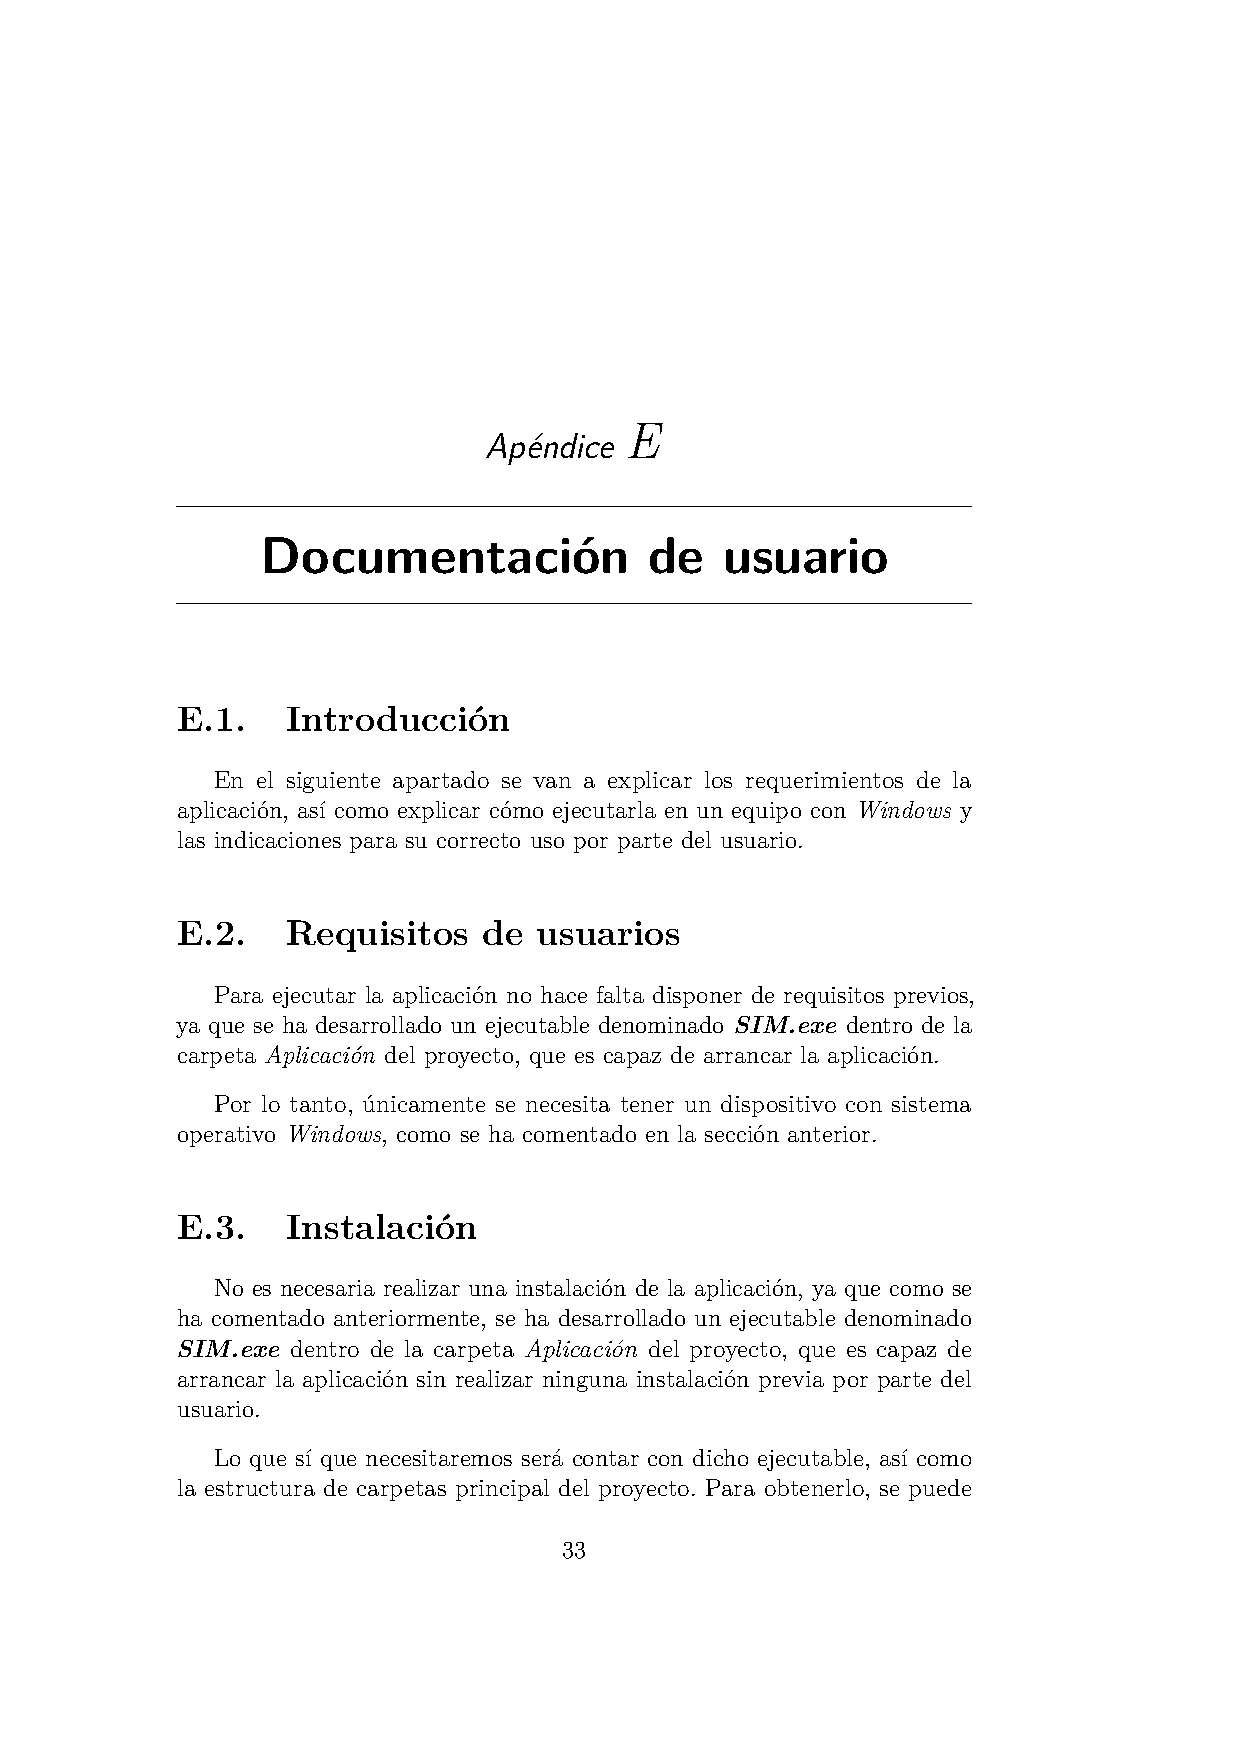
\includegraphics[width=0.8\textwidth]{ayuda}
		\caption{Opción de \emph{Ayuda}}\label{fig:ayuda}
	\end{figure}

Para finalizar, hay que comentar que la aplicación cuenta con un botón de \emph{Acerca de...}, situado a la derecha del botón de ayuda, como se aprecia en la figura \ref{fig:ayuda}.

Si pulsamos sobre este botón nos mostrará información relevante del proyecto (nombre, logotipo, autor, tutor, versión, licencia...etc) como se aprecia en la figura \ref{fig:acercaDe}.

\begin{figure}%[!h]
		\centering
		
\includegraphics[width=0.8\textwidth]{acercaDe}
		\caption{Contenido de \emph{Acerca de...}}\label{fig:acercaDe}
	\end{figure}